\documentclass[10pt]{article}
    \usepackage{tikz}
    \usetikzlibrary{arrows.meta}
    \usepackage{adjustbox}
    \usepackage{array}
    \usepackage{booktabs}
    \usepackage[landscape, margin=0.5cm]{geometry}
    \pagestyle{empty}

    \begin{document}
    \begin{center}
    \scalebox{0.7}{
    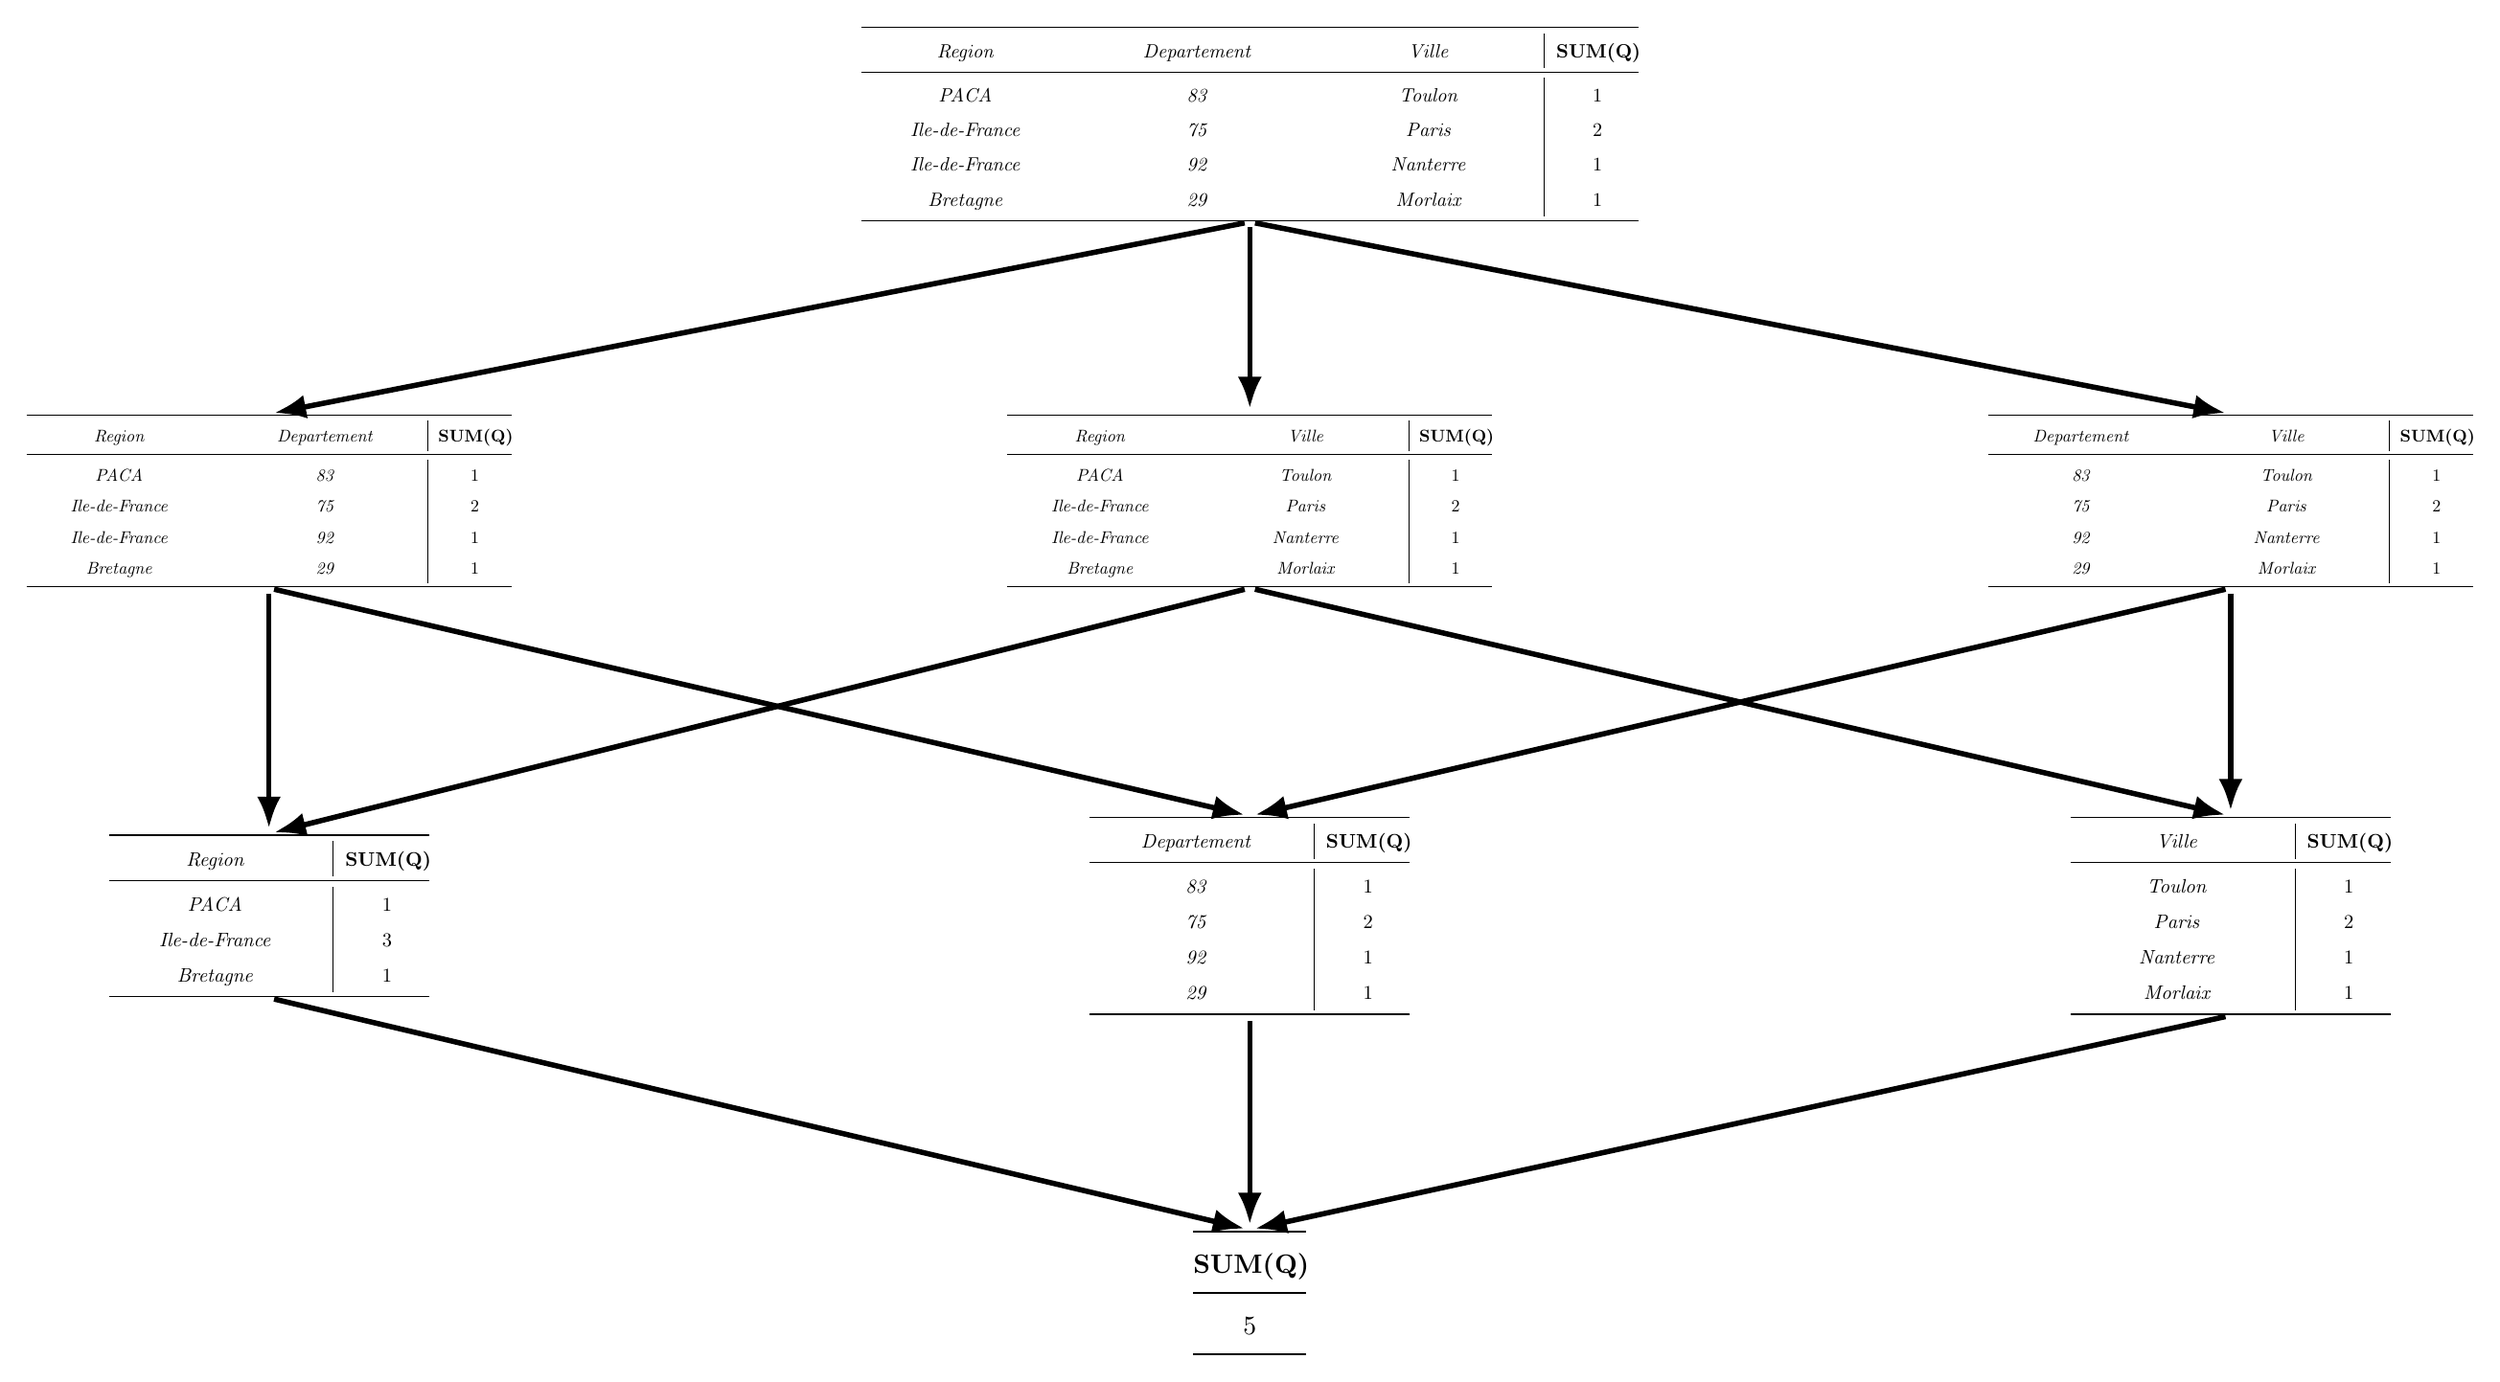
\begin{tikzpicture}[every node/.style={inner sep=0pt}]
    \newcolumntype{M}[1]{>{\centering\arraybackslash\itshape}m{#1}}
    \newcolumntype{C}[1]{>{\centering\arraybackslash}m{#1}}
    
% MAIN
\node (main) at (9,0) {
\begin{adjustbox}{max width=0.85\textwidth}
{\renewcommand{\arraystretch}{1.5}%
\begin{tabular}{@{\hspace{0pt}}M{3.8cm} M{3.8cm} M{3.8cm} !{\vrule} C{1.5cm}@{}}
\toprule
Region & Departement & Ville & \textbf{SUM(Q)} \\
\midrule
PACA & 83 & Toulon & 1 \\
Ile-de-France & 75 & Paris & 2 \\
Ile-de-France & 92 & Nanterre & 1 \\
Bretagne & 29 & Morlaix & 1 \\
\bottomrule
\end{tabular}}
\end{adjustbox}
};

% TP
\node (tp) at (-4,-5) {
\begin{adjustbox}{max width=0.53\textwidth}
{\renewcommand{\arraystretch}{1.5}%
\begin{tabular}{@{\hspace{0pt}}M{3.8cm} M{3.8cm} !{\vrule} C{1.5cm}@{}}
\toprule
Region & Departement & \textbf{SUM(Q)} \\
\midrule
PACA & 83 & 1 \\
Ile-de-France & 75 & 2 \\
Ile-de-France & 92 & 1 \\
Bretagne & 29 & 1 \\
\bottomrule
\end{tabular}}
\end{adjustbox}
};

% TE
\node (te) at (9,-5) {
\begin{adjustbox}{max width=0.53\textwidth}
{\renewcommand{\arraystretch}{1.5}%
\begin{tabular}{@{\hspace{0pt}}M{3.8cm} M{3.8cm} !{\vrule} C{1.5cm}@{}}
\toprule
Region & Ville & \textbf{SUM(Q)} \\
\midrule
PACA & Toulon & 1 \\
Ile-de-France & Paris & 2 \\
Ile-de-France & Nanterre & 1 \\
Bretagne & Morlaix & 1 \\
\bottomrule
\end{tabular}}
\end{adjustbox}
};

% PE
\node (pe) at (22,-5) {
\begin{adjustbox}{max width=0.53\textwidth}
{\renewcommand{\arraystretch}{1.5}%
\begin{tabular}{@{\hspace{0pt}}M{3.8cm} M{3.8cm} !{\vrule} C{1.5cm}@{}}
\toprule
Departement & Ville & \textbf{SUM(Q)} \\
\midrule
83 & Toulon & 1 \\
75 & Paris & 2 \\
92 & Nanterre & 1 \\
29 & Morlaix & 1 \\
\bottomrule
\end{tabular}}
\end{adjustbox}
};

% T
\node (t) at (-4,-10.5) {
\begin{adjustbox}{max width=0.35\textwidth}
{\renewcommand{\arraystretch}{1.5}%
\begin{tabular}{@{\hspace{0pt}}M{3.8cm} !{\vrule} C{1.5cm}@{}}
\toprule
Region & \textbf{SUM(Q)} \\
\midrule
PACA & 1 \\
Ile-de-France & 3 \\
Bretagne & 1 \\
\bottomrule
\end{tabular}}
\end{adjustbox}
};

% P
\node (p) at (9,-10.5) {
\begin{adjustbox}{max width=0.35\textwidth}
{\renewcommand{\arraystretch}{1.5}%
\begin{tabular}{@{\hspace{0pt}}M{3.8cm} !{\vrule} C{1.5cm}@{}}
\toprule
Departement & \textbf{SUM(Q)} \\
\midrule
83 & 1 \\
75 & 2 \\
92 & 1 \\
29 & 1 \\
\bottomrule
\end{tabular}}
\end{adjustbox}
};

% E
\node (e) at (22,-10.5) {
\begin{adjustbox}{max width=0.35\textwidth}
{\renewcommand{\arraystretch}{1.5}%
\begin{tabular}{@{\hspace{0pt}}M{3.8cm} !{\vrule} C{1.5cm}@{}}
\toprule
Ville & \textbf{SUM(Q)} \\
\midrule
Toulon & 1 \\
Paris & 2 \\
Nanterre & 1 \\
Morlaix & 1 \\
\bottomrule
\end{tabular}}
\end{adjustbox}
};

% SUM
\node (sum) at (9,-15.5) {
\begin{adjustbox}{max width=0.23\textwidth}
{\renewcommand{\arraystretch}{1.5}%
\begin{tabular}{@{}C{1.5cm}@{}}
\toprule
\textbf{SUM(Q)} \\
\midrule
5 \\
\bottomrule
\end{tabular}}
\end{adjustbox}
};
\draw[->, line width=2pt, >=Latex, shorten >=2pt, shorten <=2pt] (main.south) -- (tp.north);
\draw[->, line width=2pt, >=Latex, shorten >=2pt, shorten <=2pt] (main.south) -- (te.north);
\draw[->, line width=2pt, >=Latex, shorten >=2pt, shorten <=2pt] (main.south) -- (pe.north);
\draw[->, line width=2pt, >=Latex, shorten >=2pt, shorten <=2pt] (tp.south) -- (t.north);
\draw[->, line width=2pt, >=Latex, shorten >=2pt, shorten <=2pt] (tp.south) -- (p.north);
\draw[->, line width=2pt, >=Latex, shorten >=2pt, shorten <=2pt] (te.south) -- (t.north);
\draw[->, line width=2pt, >=Latex, shorten >=2pt, shorten <=2pt] (te.south) -- (e.north);
\draw[->, line width=2pt, >=Latex, shorten >=2pt, shorten <=2pt] (pe.south) -- (p.north);
\draw[->, line width=2pt, >=Latex, shorten >=2pt, shorten <=2pt] (pe.south) -- (e.north);
\draw[->, line width=2pt, >=Latex, shorten >=2pt, shorten <=2pt] (t.south) -- (sum.north);
\draw[->, line width=2pt, >=Latex, shorten >=2pt, shorten <=2pt] (p.south) -- (sum.north);
\draw[->, line width=2pt, >=Latex, shorten >=2pt, shorten <=2pt] (e.south) -- (sum.north);
\end{tikzpicture}
    } % ← fin de scalebox
    \end{center}
    \end{document}
    